\documentclass[11pt,a4paper]{article}
\usepackage[utf8]{inputenc}
\usepackage[T1]{fontenc}
\usepackage[margin=2.3cm]{geometry}
\usepackage{lmodern}
\usepackage{graphicx}
\usepackage{booktabs}
\usepackage{amsmath}
\usepackage{siunitx}
\usepackage{xcolor}
\usepackage{eurosym}
\usepackage{float}
\usepackage[hyphens]{url}
\usepackage[hidelinks]{hyperref}
\usepackage{caption}
\usepackage{enumitem}
\setlist{nosep, leftmargin=*}
\graphicspath{{../figures/}{figures/}}
\captionsetup{font=small, labelfont=bf}
\sisetup{group-separator={,}}
\urlstyle{same}

\title{\textbf{Is RWE on track for its 2030 coal exit?}\\[2pt]
\large Replacement ratio and delivery credibility from asset-level data}
\author{Victor Henz, Edgar Gusching, Marius Rang, Ylias Guetari\\[2pt]
\small Climate Risks (IDSI 51003), Research and Emerging Topics --- role: sustainability consultant}
\date{December 2026}

\begin{document}
\maketitle

\begin{abstract}
RWE has agreed to end lignite power generation in the Rhineland by 31 March 2030. Because the exit is fixed by law, we ask whether RWE's transition is credible as a business: does its new wind and solar replace the output of the coal it closes, and has RWE built at the pace this requires? Using the Global Energy Monitor (GEM) Global Integrated Power Tracker, corrected with public sources for ownership errors and outdated offshore statuses, we compute a capacity-factor-adjusted replacement ratio with a project-level Monte Carlo. On projects that can be identified today, the median ratio in 2030 is 0.51, so the coal output is very unlikely to be replaced; the ratio exceeds 1 only if everything planned before 2030 is built. The pace needed (about 2.2\,GW/yr) is slightly above RWE's best track record measured on a consistent basis, but within reach of its 2026 guidance. RWE's coal timeline is aligned with the IEA Net Zero milestone; what is not aligned, on identifiable projects, is the replacement.
\end{abstract}

\section{Introduction}
Phasing out coal is the first step of every 1.5\,°C pathway: the IEA Net Zero scenario phases out unabated coal in advanced economies by 2030 \cite{iea2021}, and existing fossil infrastructure already commits more emissions than a 1.5\,°C budget allows \cite{tong2019}. In Europe the question is increasingly whether the companies that close coal plants also replace them. RWE runs one of Europe's largest lignite fleets, has one of the largest renewable pipelines of any European utility, and signed a dated agreement to exit lignite by 31 March 2030 \cite{bmwk2022}, for which it receives \euro2.6\,bn of compensation \cite{ec2023}. In August 2026 the German economy ministry let its review deadline pass without deciding whether about 3\,GW of RWE lignite should be kept in a reserve until 2033 \cite{cleanthinking2026}.

Because the exit itself is legally binding, our question is about RWE's transition: (1) does its wind and solar pipeline replace the output of the coal it closes, and (2) is the required pace credible given what RWE has delivered? Our project definition (V0) stated H0: \emph{the capacity-factor-adjusted replacement ratio is $\geq 1$ by 2030 and the build rate implied by the pipeline matches RWE's history.} A probability is not a test statistic, so we evaluate H0 through two criteria set after the V0 feedback, before the final analysis:
\begin{itemize}
\item \textbf{C1 (coverage):} $P(R_{2030}\geq1)\geq0.66$ under the Current plan scenario (``likely'' on the IPCC scale);
\item \textbf{C2 (credibility):} the pace needed for $R=1$ is at most RWE's best 3-year average pace. The decisive basis is the coverage-adjusted one, the only basis on which both the need and the history are wind and solar in real GW; the GEM-visible and RWE-reported bases are reported as lower and upper bounds.
\end{itemize}
We also report H0 in its V0 wording (pace \emph{implied by} the pipeline vs history), which is a different question from C2 (pace \emph{needed}).

\section{Literature}
\paragraph{Utilities' transition and stranded assets.} Alova \cite{alova2020} analyses more than 3,000 utilities with asset-level data and finds that only about 10\% grew renewable capacity faster than fossil capacity. Pfeiffer et al.\ \cite{pfeiffer2016} show that the existing electricity capital stock already approaches the ``2\,°C capital stock'', Tong et al.\ \cite{tong2019} quantify the committed emissions of existing infrastructure, Caldecott \cite{caldecott2017} frames stranded assets as a financial and environmental risk, and Battiston et al.\ \cite{battiston2017} show how transition shocks propagate through the financial system. Our sector view follows this asset-level tradition.

\paragraph{Credibility of corporate transition plans.} Dietz et al.\ \cite{dietz2021} show that most oil and gas companies' climate goals are not Paris-aligned once intensity and scope are assessed consistently, and Rekker et al.\ \cite{rekker2023} evaluate fossil producers' production plans against 1.5\,°C pathways and find large overshoots. Our credibility test applies the same idea, announcement versus delivery, to the build-out side, with the company's own track record as reference.

\paragraph{Alignment metrics.} Our ratio belongs to the technology-share family used by PACTA \cite{pacta}. The Alignment Cookbook \cite{cookbook2020} stresses three choices we also had to make: scope (worldwide portfolio vs local), consolidation (equity vs operational control) and benchmark (company target vs external scenario). We report results for both perimeters and both consolidation rules.

\paragraph{The German coal exit.} Oei et al.\ \cite{oei2020} analyse the German phase-out and show that replacement capacity and security of supply are system questions, consistent with our finding that RWE's own pipeline replaces little of its coal output in Germany.

\section{Data and method}
\subsection{Data and audit}
Our main source is the GEM Global Integrated Power Tracker, September 2026 V2 (\num{183404} units, CC BY 4.0) \cite{gem2026}. RWE data come from its official reports and press releases \cite{rwefact2026,rwespr2023,rwe2024,rwe2025,rwe2026}, the SBTi validation \cite{sbti2025} and the IEA \cite{iea2025}. The audit leads to four corrections. (i) Only 28\% of RWE units have a parent recorded, and GEM captures about 64\% of the 18.0\,GW of wind and solar RWE reports for end 2024; we report every result on a \emph{GEM-visible} and a \emph{coverage-adjusted} basis and never compare across bases. (ii) GEM lists the Eemshaven hard-coal plant (GEM: $2\times800$\,MW; RWE quotes 1,560--1,580\,MW) under Essent/E.ON; it is RWE's \cite{rwebenelux}, so we add it back at 100\%, counting 75\% of its output as coal. (iii) GEM dates Neurath F and G to 2033 (the possible reserve) while the law says 2030; the contract is our main case. (iv) Only 34\% of RWE's pipeline MW has a start year, and several offshore statuses are out of date (Section 3.3).

\subsection{The metric and its calibration}
\begin{equation}
R_T=\frac{\sum_{i\in\text{pipeline}} B_i\,\mathrm{GW}_i\,s_i\,CF_{\text{tech}(i)}}{\sum_{j\in\text{coal}} \mathrm{GW}_j\,s_j\,c_j\,CF_{\text{coal}}},
\end{equation}
with $s$ RWE's equity share, $c_j$ the coal share of unit $j$ (0.75 for Eemshaven), $CF$ drawn from triangular ranges (low / mode / high: offshore 0.33 / 0.38 / 0.45, onshore 0.20 / 0.26 / 0.33, solar 0.09 / 0.15 / 0.22, coal 0.40 / 0.50 / 0.65) and $B_i\sim\text{Bernoulli}(p_i)$ indicating whether project $i$ is online by $T=2030$. The ratio is a \textbf{portfolio} metric (does RWE replace the output and margin it loses?); we also compute it on the Germany + Netherlands perimeter, where the coal is.

We calibrate fossil utilisation on RWE's official Scope 1 emissions (2019, 2021, 2022, 2023, 2025: 91.7, 86.9, 85.4, 61.9, 51.9\,MtCO$_2$e \cite{rwefact2026,rwespr2023}) with a regression through the origin, $\hat y=B\,x$: $B=0.92$ (90\% CI 0.83--1.02, $R^2=0.77$, $n=5$). The effective coal capacity factor is $0.50\times B=0.46$, and $B$ is drawn from its sampling distribution in the Monte Carlo. The coal output to replace is 32.1\,TWh/yr (7.9\,GW). $B$ absorbs all model error (capacity and emission factors, non-power Scope 1 sources); applying it to output as well assumes the error is mostly utilisation.

\subsection{Project probabilities}
For all projects except RWE's offshore wind we use \textbf{sector base rates} computed on all of GEM, to avoid the survival bias of rates computed on RWE's own, partly acquired, assets: construction 0.95; pre-construction with a start year $\le2030$: GEM-wide MW-weighted build rate of the technology (onshore 0.69, solar 0.73) $\times$ 0.8 for slippage; announced with a start year $\le2030$: half of that; undated: 0 (sensitivity). Multiplying $P(\text{built})\times P(\text{on time})$ assumes independence. Sector rates have their own biases: they use resolved projects only (censoring), they are global, and they ignore RWE's own delivery capacity, which is probably above average; the net effect is most likely towards caution, so we test Europe-only rates and RWE's own per-unit rate in the sensitivities.

RWE's offshore projects drive the result, so we classify each from public sources (Table~\ref{tab:off}); offshore projects without a final investment decision (FID) or with public commissioning after 2030 get $p=0$.

\begin{table}[H]
\centering\small
\begin{tabular}{p{3.4cm}p{6.0cm}ccc}
\toprule
Project & Public status (sources up to 8 Nov 2026) & COD & RWE share & $p$\\
\midrule
Sofia (UK) & under construction \cite{rweoff2026} & 2026 & 100\% & 0.95\\
Thor (DK) & under construction \cite{rwensc2025} & 2027 & 51\% & 0.95\\
Nordseecluster A (DE) & under construction, first power July 2026 \cite{rweoff2026} & 2027 & 51\% & 0.95\\
Nordseecluster B (DE) & foundations in production, COD early 2029 \cite{rweoff2026} & 2029 & 51\% & 0.85\\
OranjeWind (NL) & under construction \cite{rweoff2026} & 2027 & 50\% & 0.95\\
Norfolk Vanguard West / East (UK) & AR7 CfD; Vestas turbines contracted; FID targeted summer 2026, no public confirmation found as of 8 Nov 2026 \cite{rweAR7,rwevw2026,rweve2026} & 2029 / 2030 & 50\% & 0.60\\
Dogger Bank South, Awel y Môr (UK) & AR7 CfD, COD 2031--32 \cite{rweAR7} & 2031+ & 51 / 60\% & 0\\
Norfolk Boreas, US projects & no CfD / US offshore paused \cite{offshoremag2025} & -- & -- & 0\\
\bottomrule
\end{tabular}
\caption{RWE offshore wind projects reclassified from public sources. F.E.W.\ Baltic II (Poland) was sold to PGE and is removed. For Vanguard we use GEM's 2.8\,GW (consistent with $2\times92$ Vestas 15\,MW turbines); with the 3.1\,GW quoted at the CfD award, the ratio rises by about 0.01.}
\label{tab:off}
\end{table}

\subsection{Scenarios and uncertainty}
\emph{Track record}: RWE adds wind and solar as in 2016--2025 (bootstrap of yearly additions). \emph{Current plan}: each project is drawn with the probability above; the sector rates, the offshore probabilities and $B$ are themselves uncertain. \emph{Full delivery}: everything with a planned start before 2030 is built, plus undated onshore and solar at 0.8. These are our own delivery hypotheses, not IEA scenarios. Projects share risks (supply chains, auctions, rates), so outcomes are drawn through a Gaussian copula with a common shock per group ($\rho=0.5$ offshore, $0.3$ onshore/solar). We run \num{5000} draws and report probabilities rounded to 0.05 with IPCC likelihood terms.

\section{Sector view}
Europe (EU-27, UK, Norway, Switzerland) still operates 77.5\,GW of coal, 70\% in Germany and Poland. If all GEM retirement dates are respected, 43\% closes by 2030. At \euro100/t the fleet's carbon bill is about \euro35\,bn a year, and RWE's Niederaussem and Neurath plants rank fourth and fifth by carbon cost. Fig.~\ref{fig:sector}a shows the gap in TWh between expected new wind and solar and coal output by country: Germany and Poland have by far the largest shortfall. Among utilities (European assets only, same uncalibrated coal capacity factor for all, Fig.~\ref{fig:sector}b), the Central European coal owners have almost no dated pipeline; RWE has the largest expected new output among coal owners but, on its European assets alone, it covers only about a fifth of its coal output.

\begin{figure}[H]
\centering
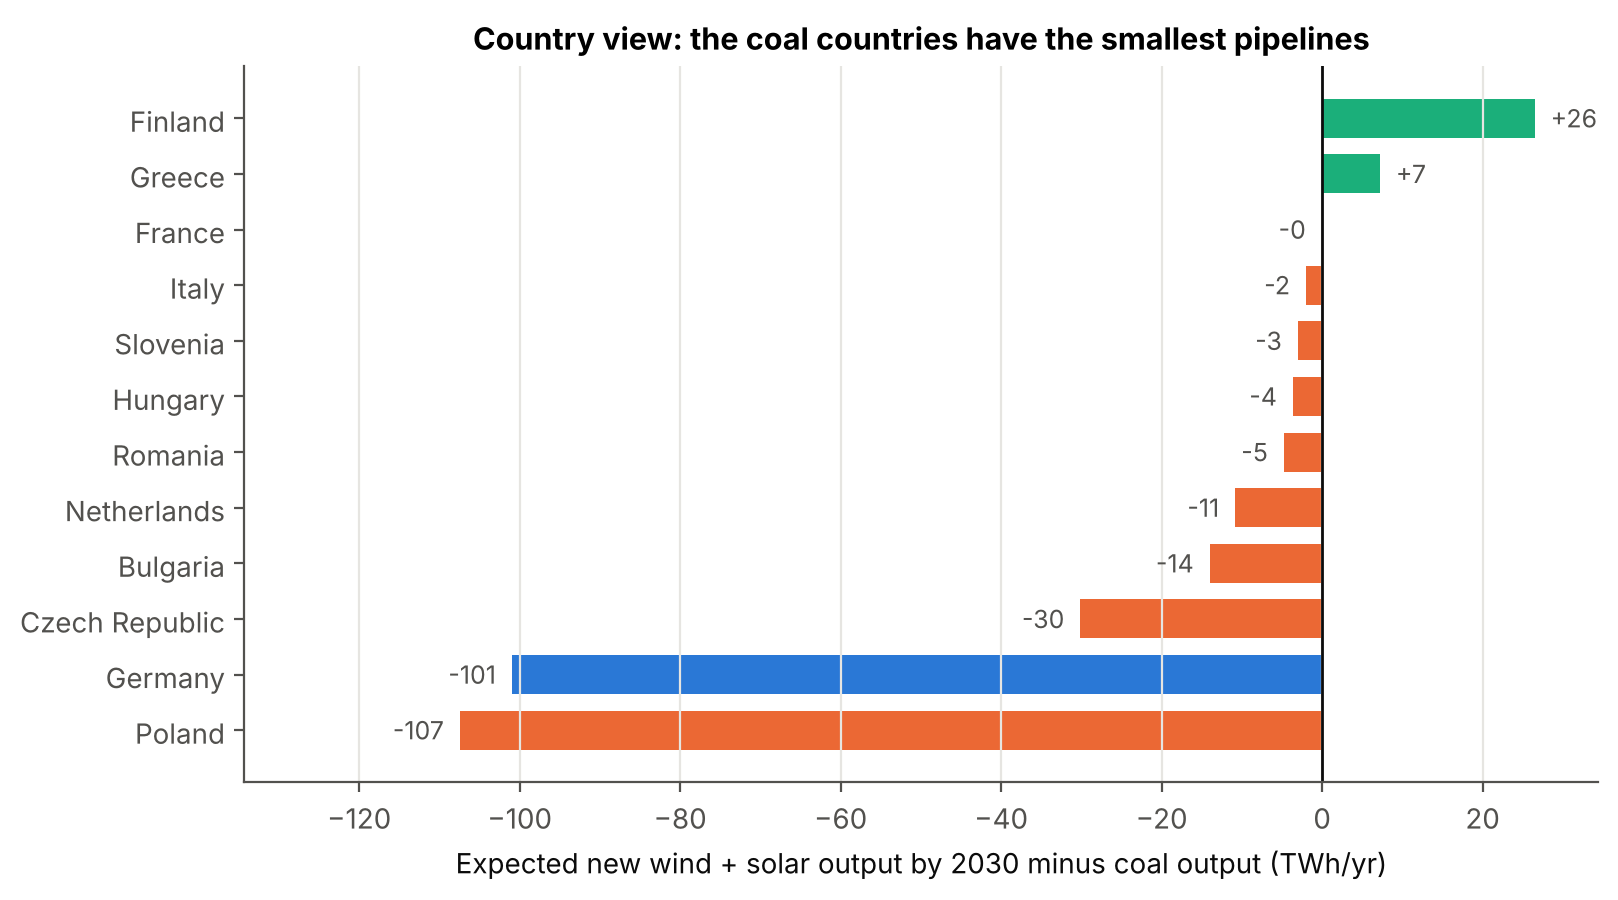
\includegraphics[width=0.49\linewidth]{s1_country_gap.png}\hfill
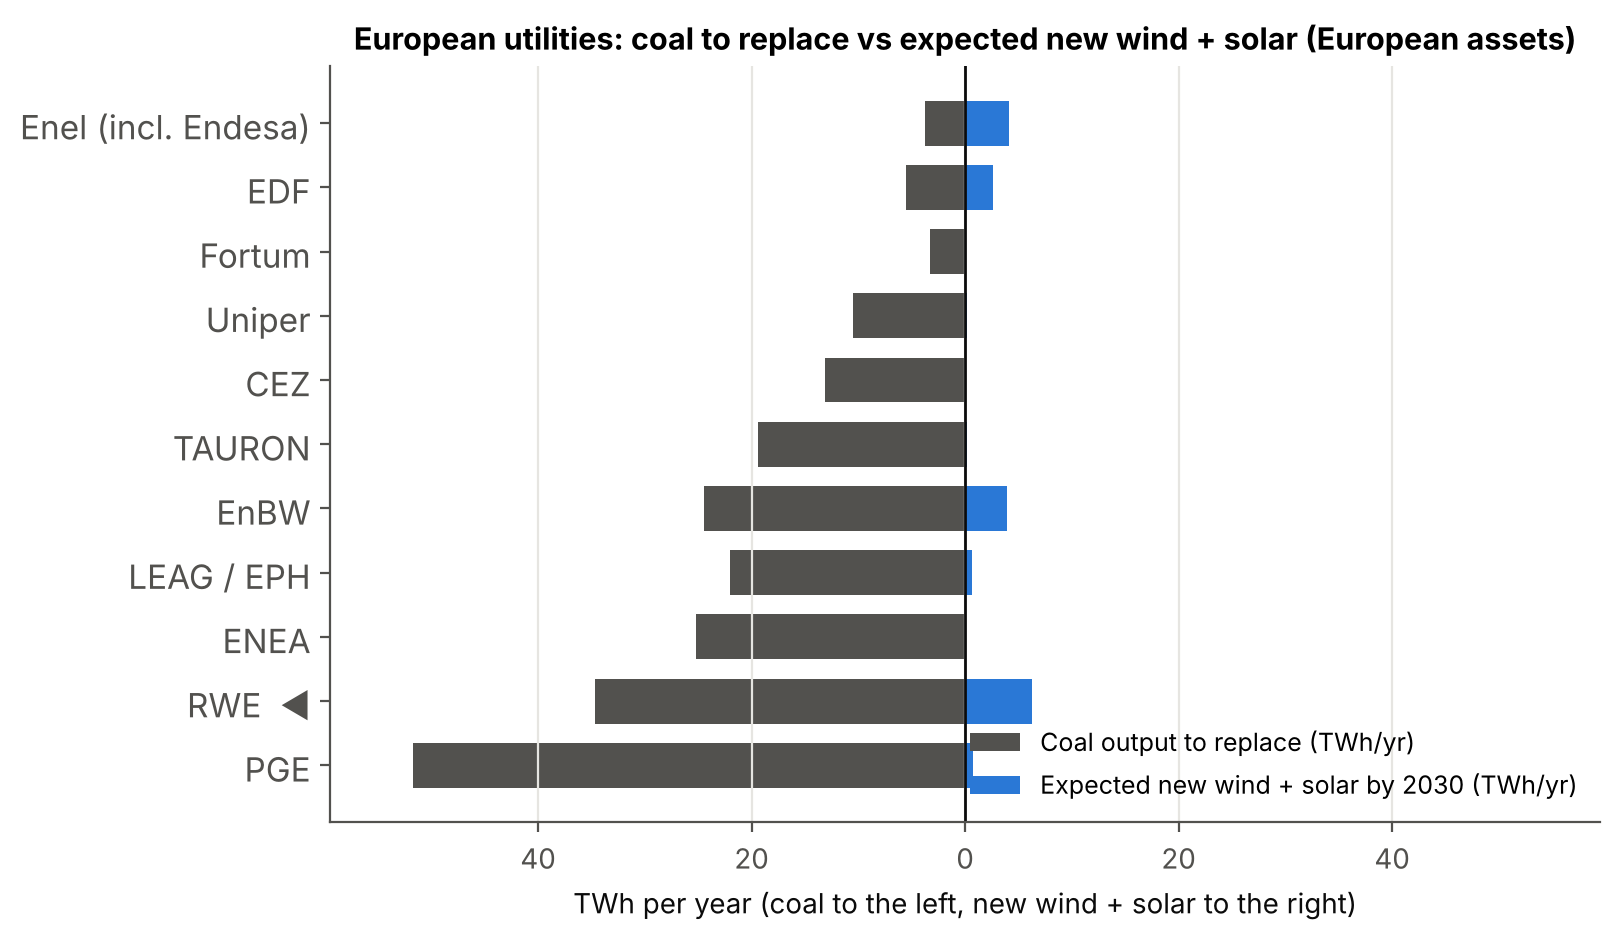
\includegraphics[width=0.49\linewidth]{s1_peers.png}
\caption{(a) Expected new wind + solar output by 2030 minus coal output, by country (TWh/yr). (b) European utilities, European assets only: coal output vs expected new wind + solar output.}
\label{fig:sector}
\end{figure}

\section{Results for RWE}
\subsection{History, pipeline and the bridge from earlier estimates}
RWE's wind and solar additions visible in GEM averaged 0.78\,GW/yr over 2016--2025, with a best 3-year average of 1.26\,GW/yr (2021--23); coverage-adjusted, 1.22 and 1.95\,GW/yr. RWE reports about 2.0\,GW commissioned in 2024 and 2.8\,GW in 2025, across all technologies including batteries (Fig.~\ref{fig:hist}a). Of 27.1\,GW (equity) of pipeline in GEM, 5.7\,GW is expected online by 2030 in the Current plan, 3.7\,GW of it offshore and only 1.1\,GW in Germany and the Netherlands (Fig.~\ref{fig:hist}b).

\begin{figure}[H]
\centering
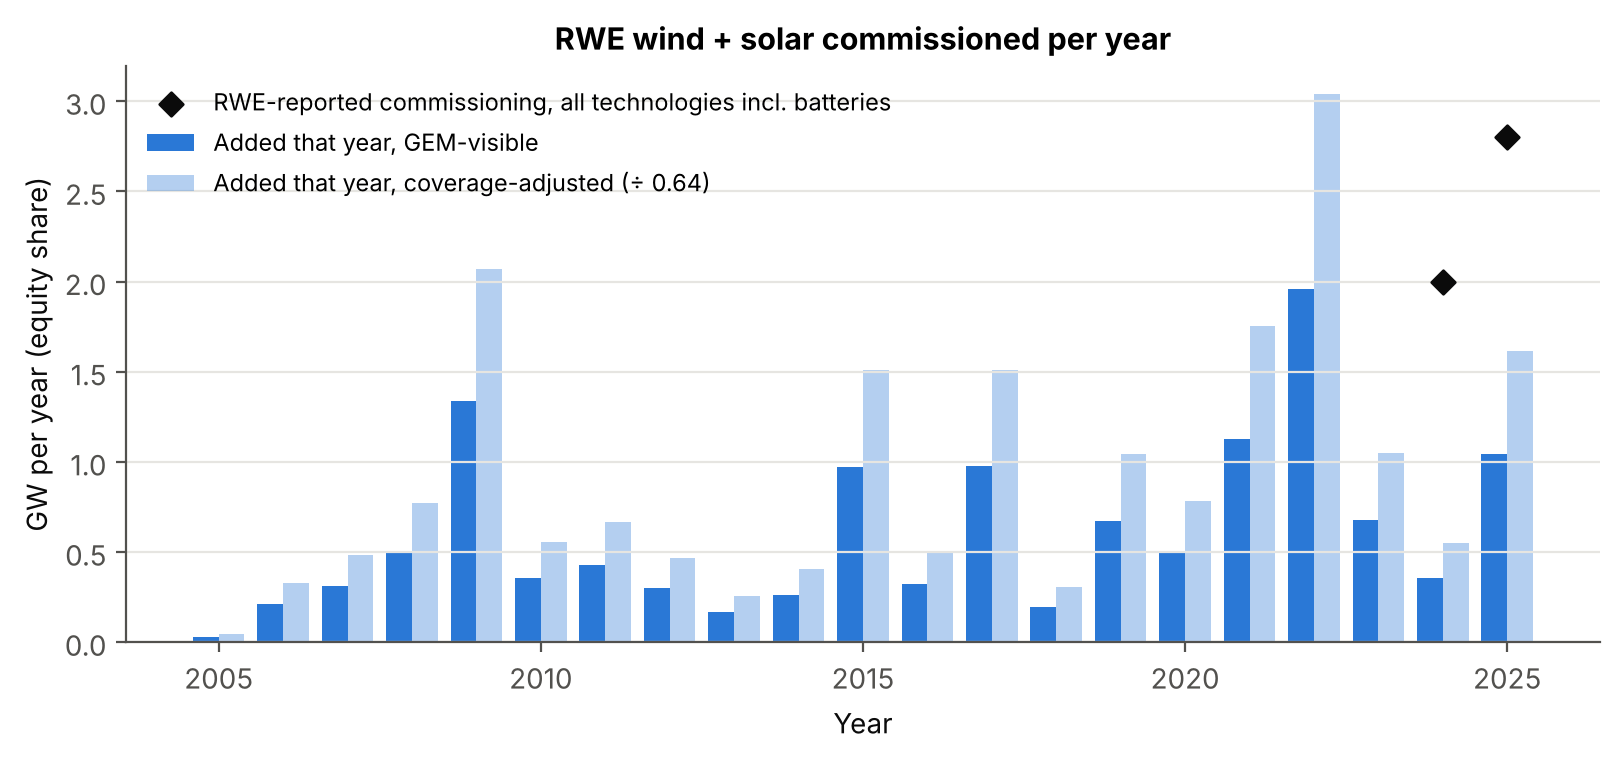
\includegraphics[width=0.52\linewidth]{r2_history.png}\hfill
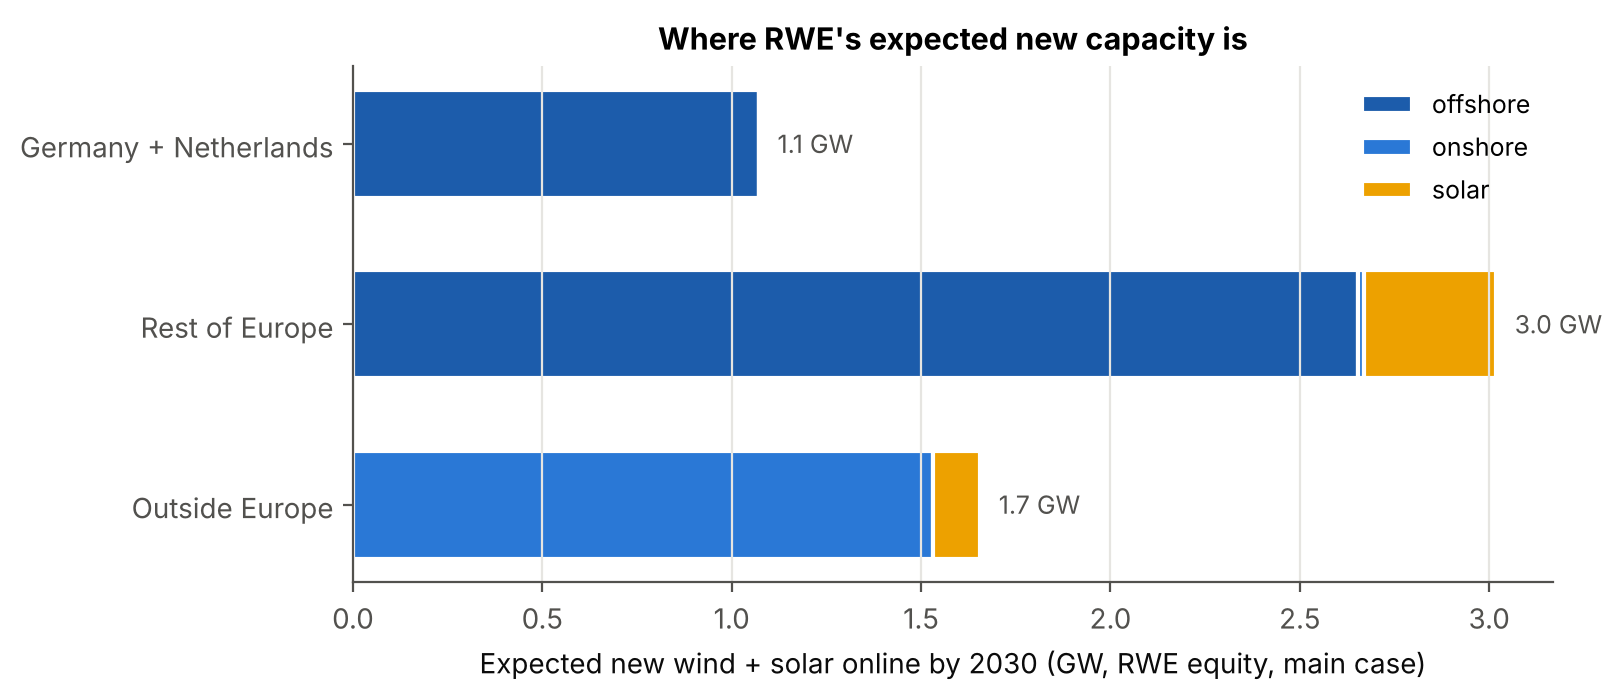
\includegraphics[width=0.46\linewidth]{r5_pipeline_composition.png}
\caption{(a) Wind + solar commissioned per year: GEM-visible, coverage-adjusted, and RWE-reported (all technologies). (b) Expected new capacity by 2030 by region and technology (Current plan).}
\label{fig:hist}
\end{figure}

Our Lab 5 gave a median ratio of 1.10. Table~\ref{tab:bridge} explains the move to the current estimate in expected value, one documented correction at a time. Adding Eemshaven and replacing RWE-specific stage rates by sector rates are the largest downward steps; the calibration and the offshore evidence (several projects are further advanced than GEM shows) move the ratio up. Excluding undated projects is a choice that makes the main case a lower bound.

\begin{table}[H]
\centering\small
\begin{tabular}{lcc}
\toprule
Step (cumulative) & Expected ratio & Change\\
\midrule
Lab 5 logic, no Eemshaven (Lab 5 Monte Carlo median 1.10) & 1.19 & \\
+ Eemshaven added to the coal & 1.01 & $-0.18$\\
+ coal capacity factor calibrated on reported emissions & 1.09 & $+0.08$\\
+ sector build rates instead of RWE-specific rates & 0.52 & $-0.57$\\
+ undated projects excluded & 0.30 & $-0.22$\\
+ offshore projects from public evidence (current main case) & 0.52 & $+0.22$\\
\bottomrule
\end{tabular}
\caption{Bridge from the Lab 5 estimate to the current main case (expected values; the Current plan Monte Carlo median is 0.51).}
\label{tab:bridge}
\end{table}

\subsection{Replacement ratio and criterion C1}
\begin{table}[H]
\centering\small
\begin{tabular}{llccc}
\toprule
Scenario & Basis & New GW 2030 & Ratio median [90\% int.] & $P(R\ge1)$\\
\midrule
Track record & GEM-visible & 3.8 & 0.34 [0.19--0.54] & $\approx0$\\
Current plan & GEM-visible & 5.8 & 0.51 [0.31--0.72] & $\approx0$\\
Full delivery & GEM-visible & 12.2 & 1.02 [0.70--1.32] & $\approx0.55$\\
Track record & coverage-adjusted & 6.0 & 0.52 [0.30--0.84] & $\approx0$\\
Current plan & coverage-adjusted & 6.8 & 0.57 [0.34--0.84] & $\approx0$\\
Full delivery & coverage-adjusted & 15.5 & 1.22 [0.84--1.60] & $\approx0.85$\\
\bottomrule
\end{tabular}
\caption{Replacement ratio in 2030 (portfolio perimeter). On the Germany + Netherlands perimeter the expected ratio is 0.11.}
\label{tab:scen}
\end{table}

C1 is not met under the Current plan on either basis (Table~\ref{tab:scen}, Fig.~\ref{fig:scen}). It is met under Full delivery on the coverage-adjusted basis (``likely''), and close to the threshold on the GEM basis (``about as likely as not''): C1 fails because of what cannot yet be identified, not because the announced plan is too small. Counting only capacity online before 31 March 2030 lowers the median to 0.47.

\begin{figure}[H]
\centering
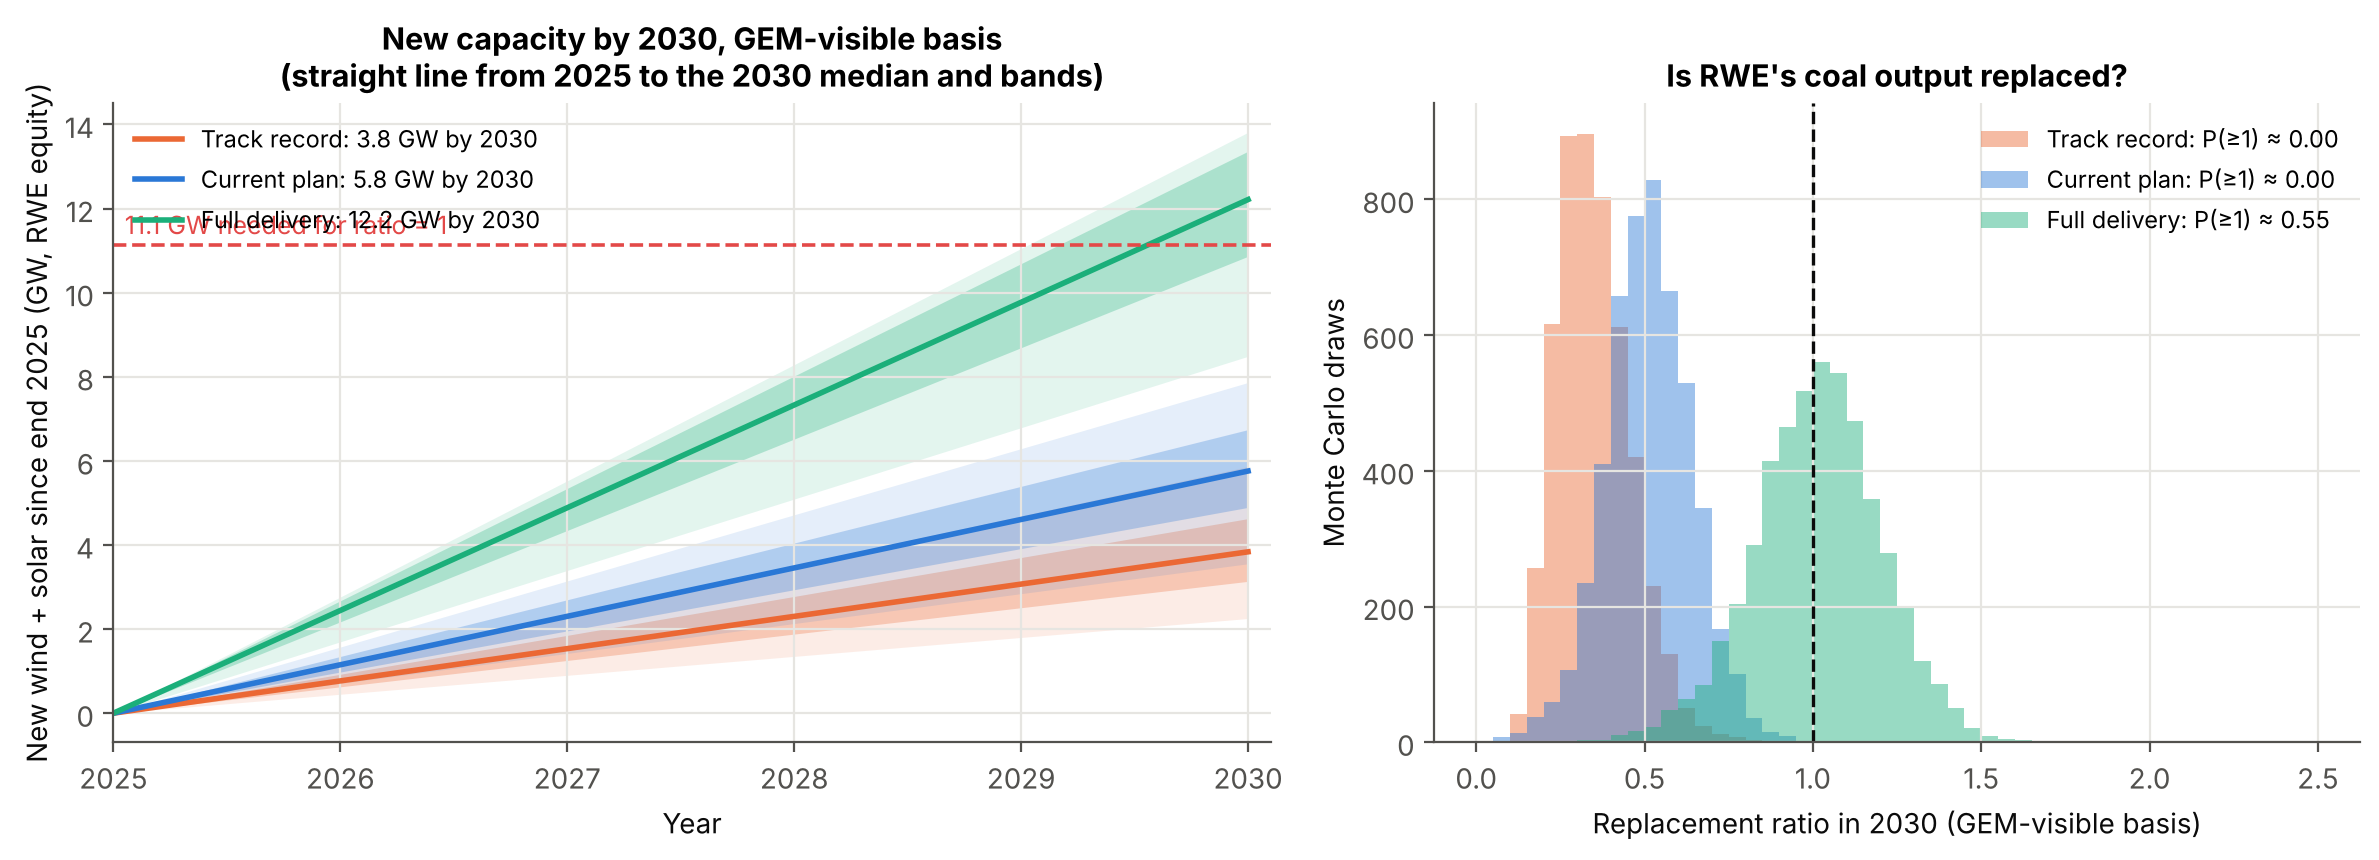
\includegraphics[width=\linewidth]{r3_scenarios.png}
\caption{Left: new wind + solar capacity since end 2025 (GEM-visible basis); lines are straight interpolations between 2025 and the 2030 median and bands, not modelled yearly paths. Right: distribution of the 2030 replacement ratio.}
\label{fig:scen}
\end{figure}

\subsection{Criterion C2 and RWE's strategy}
A ratio of 1 needs 11.1\,GW of new wind and solar, i.e.\ 2.2\,GW/yr to the end of 2030 (2.6\,GW/yr to be online before 31 March 2030). On the decisive coverage-adjusted basis this is $1.14\times$ RWE's best 3-year average, so \textbf{C2 narrowly fails}. The bounds are $1.78\times$ (GEM-visible) and $0.93\times$ (RWE-reported 2024--25, including batteries). The best 3-year average includes acquired assets; removing all US assets commissioned before 2023 (largely acquired with E.ON's portfolio in 2019 and Con Edison Clean Energy in 2023) lowers it and raises the factor to $1.9\times$. Comparing a physical need with GEM-visible history alone would overstate the gap, which is why the decisive basis matters.

In the V0 wording of H0, the pace implied by the identifiable pipeline (1.15\,GW/yr) is within RWE's GEM-visible history (0.78--1.26\,GW/yr), so this part of H0 holds: RWE is not planning to build faster than it has, it has too little that can be identified. RWE cut its 2025--2030 net investment plan by \euro10\,bn to \euro35\,bn in March 2025 and paused its US offshore activities \cite{rwe2025,offshoremag2025}; in March 2026 it guided to about 65\,GW by 2031, of which about 19\,GW outside German flexible generation, i.e.\ about 3.2\,GW/yr including batteries \cite{rwe2026}. If all of it were wind and solar, the 2030 ratio would be about 1.4. The difference between this guidance and the 1.2\,GW/yr supported by named, dated projects is where the credibility risk lies.

\subsection{Benchmarks}
On coal, RWE's timeline is aligned with the IEA Net Zero milestone of phasing out unabated coal in advanced economies by 2030 \cite{iea2021}. For renewables, we apply IEA multipliers pro rata to RWE's 2022 wind and solar capacity: $\times2.49$ (IEA Renewables 2025 main case, 9,530\,GW), $\times2.72$ (accelerated case) and $\times3$ (tripling, about 11,500\,GW according to the IEA) \cite{iea2025}, i.e.\ 26.4, 28.8 and 31.8\,GW on the GEM basis. No scenario reaches even the main case (Current plan 18.0\,GW, Full delivery 24.4\,GW). These multipliers cover all renewables, including slow-growing hydro, and are global; a European per-technology trajectory, as in PACTA, would be a better yardstick and is left for future work.

\subsection{Sensitivities}
\begin{figure}[H]
\centering
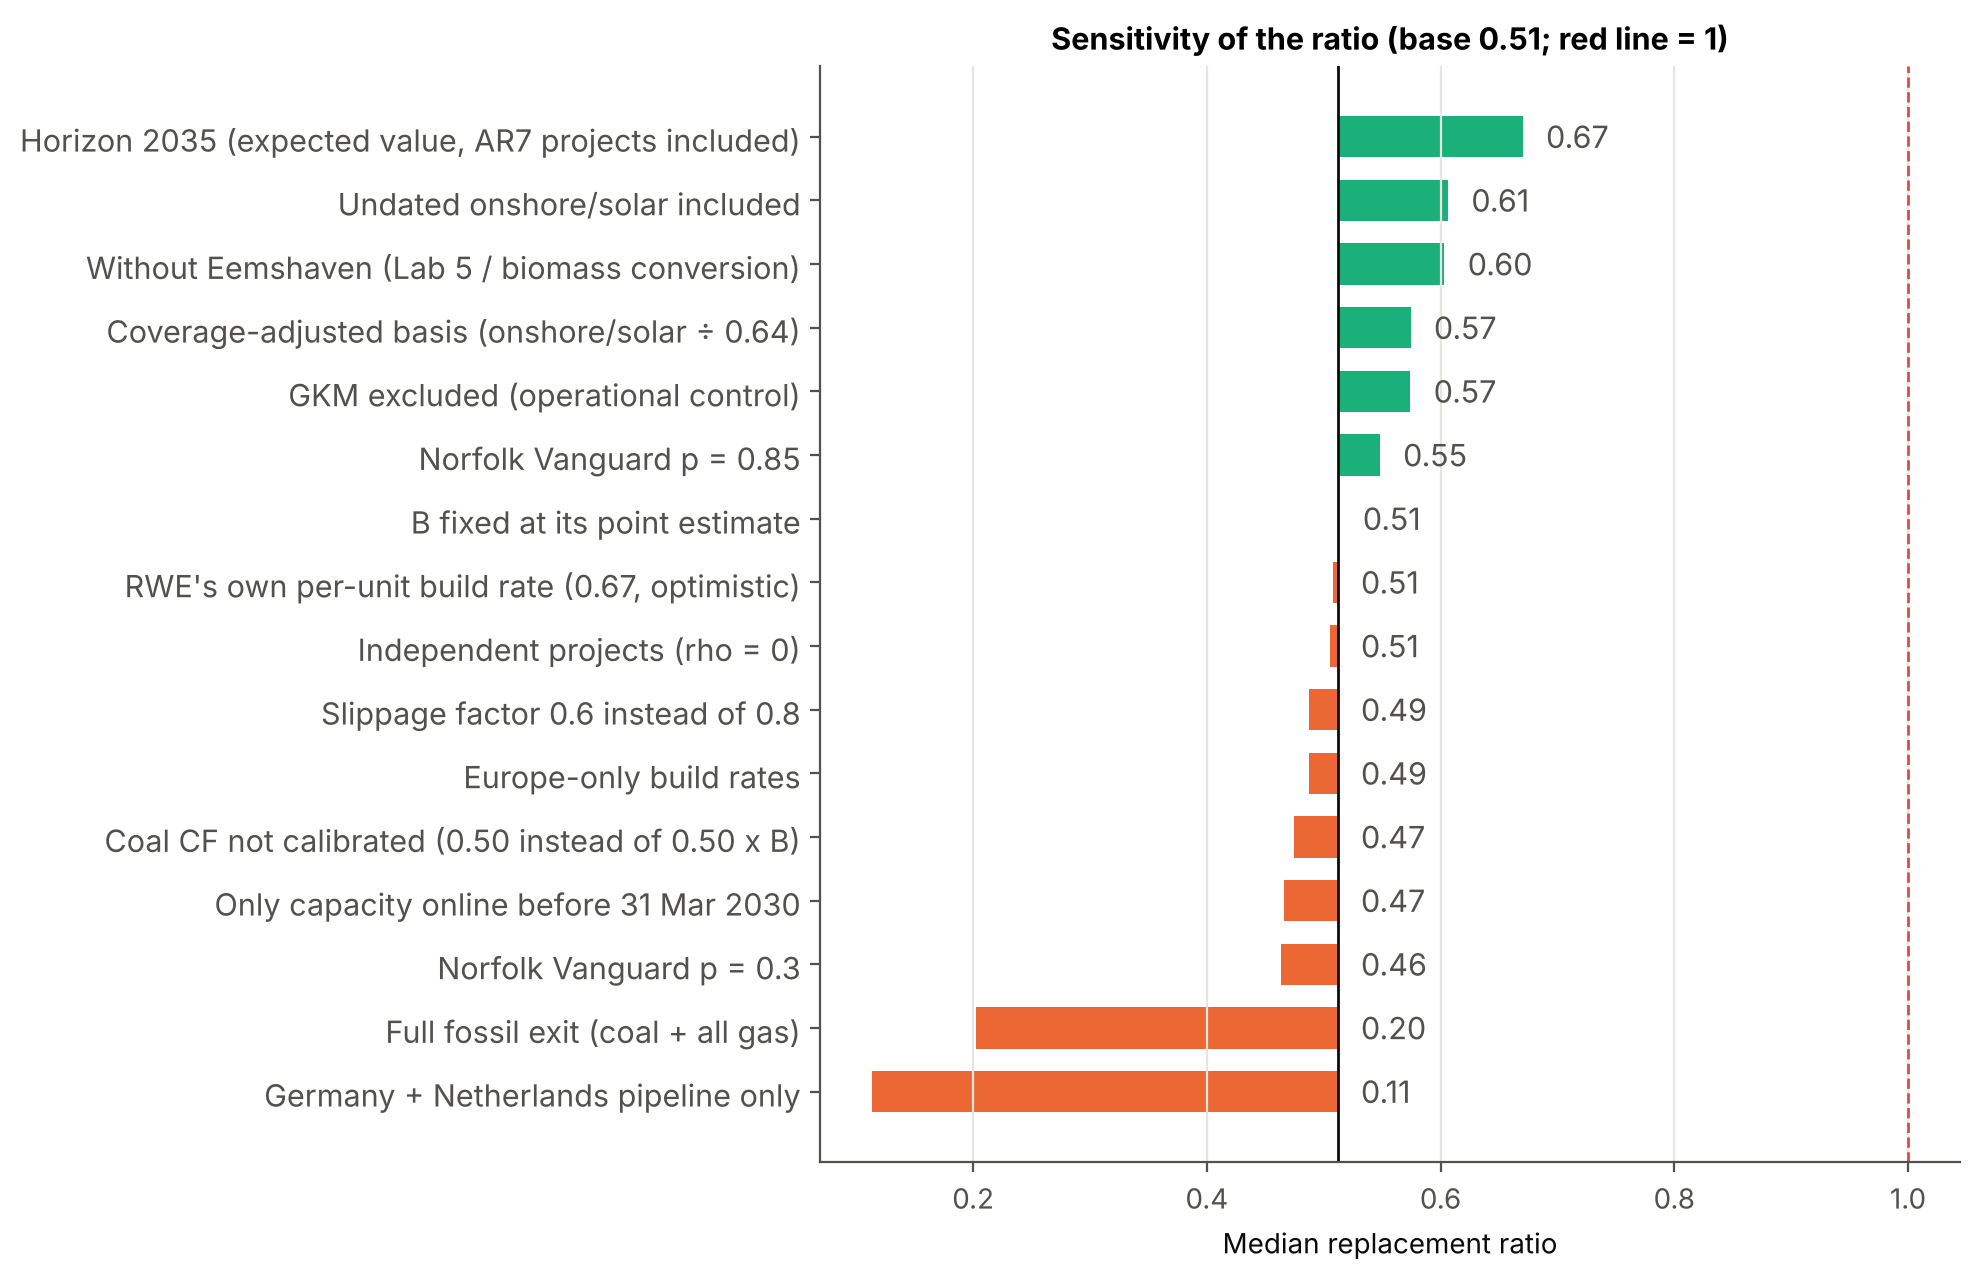
\includegraphics[width=0.85\linewidth]{r4_tornado.png}
\caption{Median replacement ratio under one-at-a-time changes (Current plan, GEM-visible basis).}
\label{fig:tornado}
\end{figure}
No single assumption brings the Current plan to 1 (Fig.~\ref{fig:tornado}). Including undated onshore and solar gives 0.61, removing Eemshaven 0.60, Europe-only or RWE-specific build rates 0.49--0.51, and the plausible range for Norfolk Vanguard 0.46--0.55. With a 2035 horizon (Dogger Bank South and Awel y Môr included) the expected ratio is 0.67. A full fossil exit (coal and 15.7\,GW of gas) gives 0.20.

\section{Extensions}
\paragraph{SBTi intensity.} RWE's SBTi-validated target is $-71.1\%$ Scope 1+2 emissions per MWh by 2030 versus 2022 \cite{sbti2025}. RWE publishes 0.55\,tCO$_2$e/MWh for 2022 (0.48 in 2023, 0.43 in 2025) \cite{rwespr2023,rwefact2026}, so the 2030 target is 0.159. Our model reproduces the published 2025 intensity well (0.44 vs 0.43). \textbf{Under our model assumptions}, the 2030 intensity is 0.22\,tCO$_2$e/MWh under the Current plan and 0.19 under Full delivery with coal closed on time, and higher with a reserve (Fig.~\ref{fig:emis}). The driver is the gas fleet: at a gas capacity factor of 0.30 the intensity is still about 0.18. This rests on a five-point calibration and constant gas utilisation, so we read it as ``the target requires lower gas utilisation or more renewables than our scenarios contain'' rather than as a firm prediction.

\begin{figure}[H]
\centering
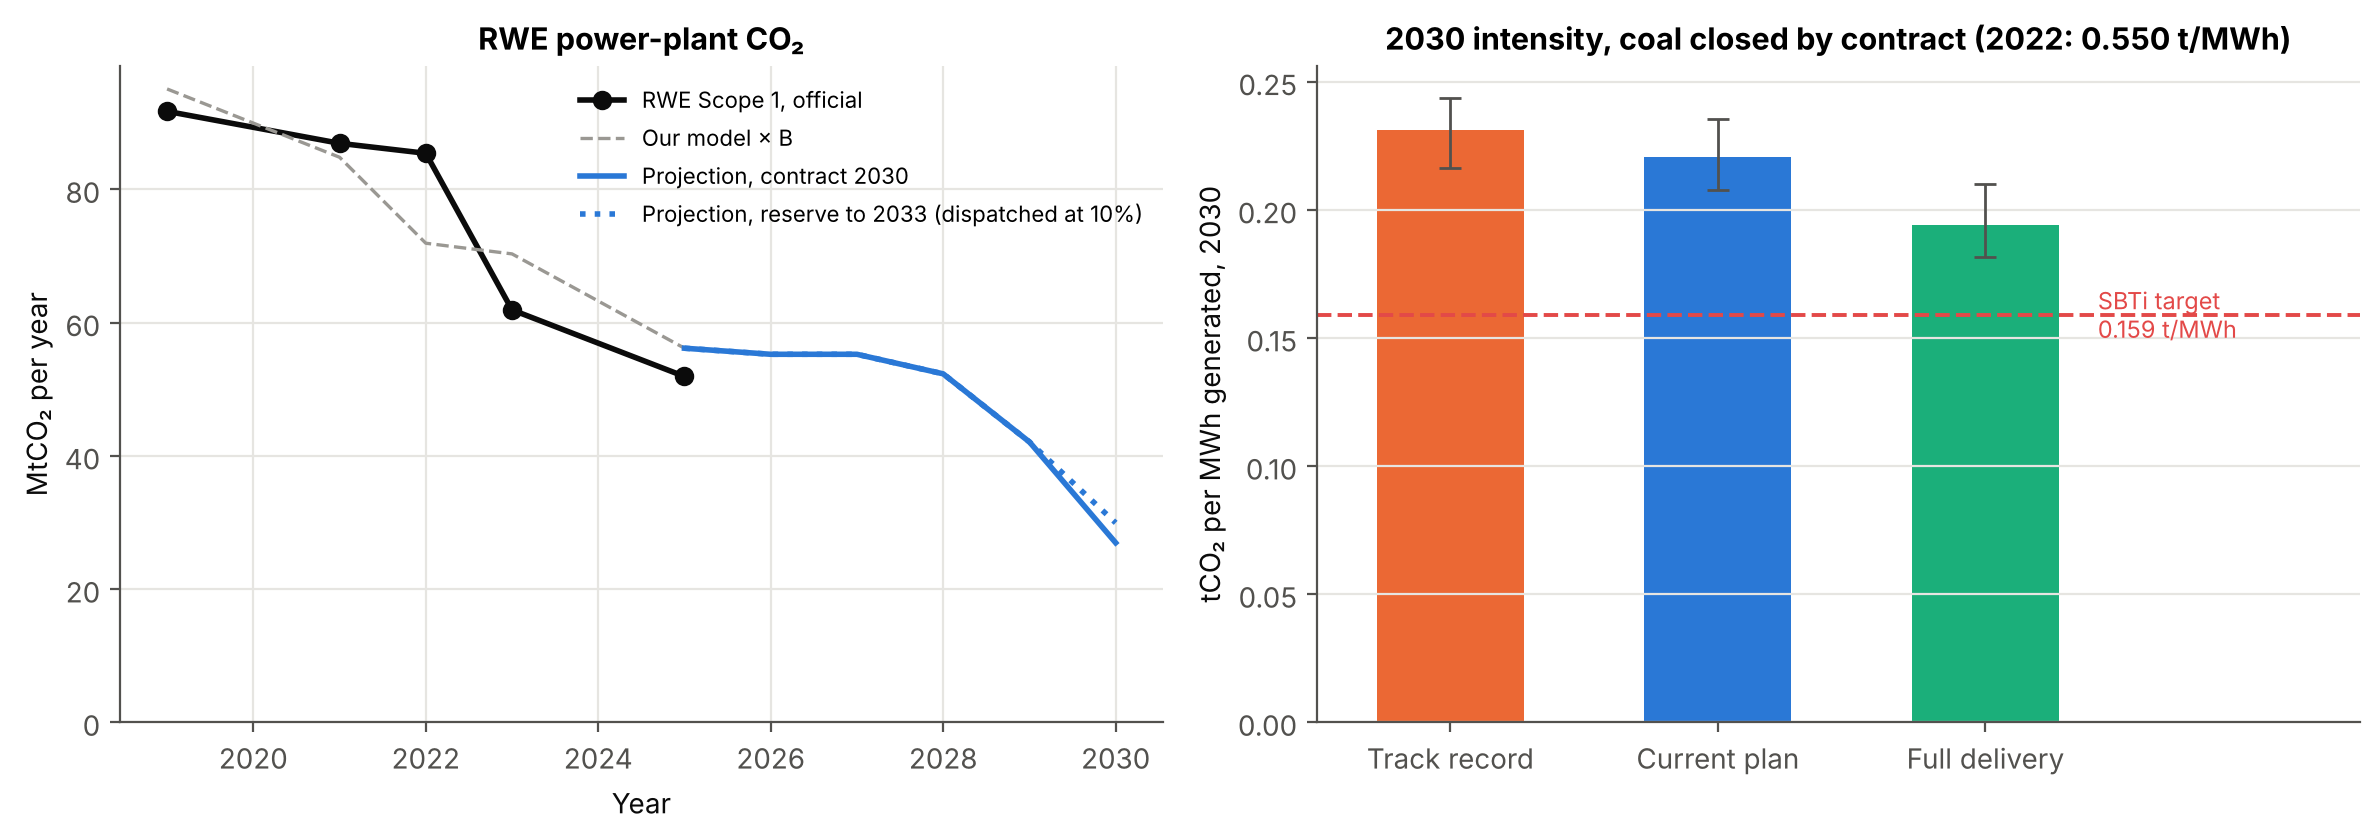
\includegraphics[width=\linewidth]{g1_emissions_intensity.png}
\caption{Left: RWE's official Scope 1 emissions, our calibrated model and the Current plan projection. Right: 2030 intensity vs the SBTi target (coal closed by contract).}
\label{fig:emis}
\end{figure}

\paragraph{Carbon cost relative to EBITDA.} The course guidelines call carbon cost / company value a ``Climate VaR''; what we compute is a flow ratio, not a quantile of a loss distribution. RWE's 2025 gross carbon cost equals 83\% of its adjusted EBITDA at \euro82/t; with coal closed it falls to about 34\% of 2027 guided EBITDA. EBITDA is already net of carbon costs that are largely passed into power prices, the price path is flat, hedging is ignored, and the \euro2.6\,bn compensation is not included.

\paragraph{Firm capacity.} With de-rating factors in the range proposed for the GB Capacity Market (offshore 12--15\%, onshore 8--9\%, solar 1--2\% \cite{ngdrf}), used as a proxy for lack of German equivalents, and 0.90 for thermal plants, RWE loses about 7.1\,GW of firm capacity in Germany and the Netherlands; its own new wind, solar and gas there replace about 1.7\,GW. The remaining gap is a system question, which is why a reserve is being discussed.

\section{Uncertainty and limitations}
(i) Ownership coverage and an undated pipeline: the main case is a lower bound by construction. (ii) Sector rates, the 0.8 slippage factor, the offshore probabilities and the correlations are assumptions. (iii) The calibration uses five points; $B$ is drawn in the Monte Carlo, but its use on output assumes the error is mostly utilisation. (iv) In our back-test (Lab 5), even the best simple model covered only 67\% of outcomes three years ahead with a nominal 90\% band, and a naive drift had the best interval score \cite{gneiting2007}; our intervals are therefore probably still too narrow. (v) The history is a back-projection that includes acquisitions. (vi) The metric is in energy and says nothing about firm capacity.

\section{Conclusion and recommendations}
On identifiable projects, H0 cannot be supported: C1 fails, and C2 narrowly fails on the decisive basis. Two qualifications matter: in its V0 wording the build-rate part of H0 holds, and C1 is met if everything planned before 2030 is built. RWE's coal timeline is NZE-aligned; the replacement is not, on the projects visible today. We recommend that investors judge RWE on named, dated projects (FID of Norfolk Vanguard, progress of Nordseecluster B, commissioned GW per year against about 2.2\,GW/yr); that RWE publish a dated project list and a plan for gas utilisation consistent with its SBTi target; and that policymakers treat post-2030 firm capacity as a system issue to be solved by timely flexibility tenders rather than a lignite reserve.

\paragraph{Changes since the project definition.} The denominator is the coal RWE committed to close rather than coal, gas and oil (RWE has no dated gas exit; full fossil exit is a sensitivity); we use equity share and report operational control as a sensitivity; we use GEM September 2026 V2; ENTSO-E capacity factors were replaced by calibration on reported emissions and generation because we could not set up the ENTSO-E API in time; and H0 is evaluated through criteria set after the V0 feedback.

\paragraph{Use of AI tools.} We used an AI assistant (Claude, Anthropic) to help write and debug code, draft text, and build the dashboard and website. Modelling choices, sources and results were checked by the team.

\paragraph{Reproducibility.} Code and data processing are in the project repository:
\begin{itemize}
\item notebook: \path{notebooks/RWE_coal_exit_final_project.ipynb}
\item app: \path{app/streamlit_app.py}; website: \path{docs/index.html}
\end{itemize}

\begin{thebibliography}{99}\small\sloppy
\bibitem{alova2020} Alova, G. (2020). A global analysis of the progress and failure of electric utilities to adapt their portfolios of power-generation assets to the energy transition. \emph{Nature Energy}, 5, 920--927. \url{https://doi.org/10.1038/s41560-020-00686-5}
\bibitem{battiston2017} Battiston, S., Mandel, A., Monasterolo, I., Schütze, F. and Visentin, G. (2017). A climate stress-test of the financial system. \emph{Nature Climate Change}, 7, 283--288. \url{https://doi.org/10.1038/nclimate3255}
\bibitem{caldecott2017} Caldecott, B. (2017). Introduction to special issue: stranded assets and the environment. \emph{Journal of Sustainable Finance \& Investment}, 7(1), 1--13. \url{https://doi.org/10.1080/20430795.2016.1266748}
\bibitem{dietz2021} Dietz, S., Gardiner, D., Jahn, V. and Noels, J. (2021). How ambitious are oil and gas companies' climate goals? \emph{Science}, 374(6566), 405--408. \url{https://www.lse.ac.uk/granthaminstitute/publication/how-ambitious-are-oil-and-gas-companies-climate-goals/}
\bibitem{gneiting2007} Gneiting, T. and Raftery, A. E. (2007). Strictly proper scoring rules, prediction, and estimation. \emph{Journal of the American Statistical Association}, 102(477), 359--378. \url{https://doi.org/10.1198/016214506000001437}
\bibitem{oei2020} Oei, P.-Y., Hermann, H., Herpich, P., Holtemöller, O., Lünenbürger, B. and Schult, C. (2020). Coal phase-out in Germany -- Implications and policies for affected regions. \emph{Energy}, 196, 117004. \url{https://doi.org/10.1016/j.energy.2020.117004}
\bibitem{pfeiffer2016} Pfeiffer, A., Millar, R., Hepburn, C. and Beinhocker, E. (2016). The `2°C capital stock' for electricity generation. \emph{Applied Energy}, 179, 1395--1408. \url{https://doi.org/10.1016/j.apenergy.2016.07.074}
\bibitem{rekker2023} Rekker, S., Chen, G., Heede, R., Ives, M. C., Wade, B. and Greig, C. (2023). Evaluating fossil fuel companies' alignment with 1.5\,°C climate pathways. \emph{Nature Climate Change}, 13(9), 927--934. \url{https://doi.org/10.1038/s41558-023-01734-0}
\bibitem{tong2019} Tong, D. et al. (2019). Committed emissions from existing energy infrastructure jeopardize 1.5\,°C climate target. \emph{Nature}, 572, 373--377. \url{https://doi.org/10.1038/s41586-019-1364-3}
\bibitem{cookbook2020} Institut Louis Bachelier et al. (2020). \emph{The Alignment Cookbook}. \url{https://institutlouisbachelier.org/en/report-portfolios-alignment-with-low-carbon-trajectories} (accessed 8 Nov 2026).
\bibitem{pacta} RMI. \emph{PACTA methodology}. \url{https://pacta.rmi.org} (accessed 8 Nov 2026).
\bibitem{iea2021} IEA (2021). \emph{Net Zero by 2050: A Roadmap for the Global Energy Sector}. \url{https://www.iea.org/reports/net-zero-by-2050}
\bibitem{iea2025} IEA (2025). \emph{Renewables 2025}. \url{https://www.iea.org/reports/renewables-2025} (accessed 8 Nov 2026).
\bibitem{gem2026} Global Energy Monitor (2026). \emph{Global Integrated Power Tracker}, September 2026 V2, CC BY 4.0. \url{https://globalenergymonitor.org/projects/global-integrated-power-tracker/}
\bibitem{bmwk2022} BMWK, MWIKE NRW and RWE (2022). Agreement on an accelerated coal phase-out in 2030, 4 October 2022.
\bibitem{ec2023} RWE AG (2023). European Commission approves compensation for early phase-out of coal, 11 December 2023. \url{https://www.rwe.com/en/press/rwe-ag/2023-12-11-european-commission-approves-compensation-for-early-phase-out-of-coal} (accessed 8 Nov 2026).
\bibitem{cleanthinking2026} Clean Thinking (2026). Braunkohleausstieg 2030 in NRW: Streit um drei Blöcke, 13 August 2026. \url{https://www.cleanthinking.de/?p=1071261} (accessed 8 Nov 2026).
\bibitem{rwefact2026} RWE AG (2026). \emph{Factbook 2026}, pp.\ 12--13. \url{https://www.rwe.com/-/media/RWE/documents/05-investor-relations/finanzkalendar-und-veroeffentlichungen/veroeffentlichungen-und-praesentationen/RWE-Factbook-2026.pdf} (accessed 8 Nov 2026).
\bibitem{rwespr2023} RWE AG (2024). \emph{Sustainability Performance Report 2023}. \url{https://www.rwe.com/-/media/RWE/documents/09-verantwortung-nachhaltigkeit/cr-berichte/sustainability-performance-report-2023.pdf} (accessed 8 Nov 2026).
\bibitem{rwe2024} RWE AG (2024). RWE significantly expands its green portfolio in fiscal 2023, 14 March 2024. \url{https://www.rwe.com/en/press/rwe-ag/2024-03-14-rwe-significantly-expands-its-green-portfolio-in-fiscal-2023/} (accessed 8 Nov 2026).
\bibitem{rwe2025} RWE AG (2025). Full-year results 2024 and investment plan, 20 March 2025. \url{https://www.rwe.com/en/investor-relations/financial-calendar-and-publications/news-and-ad-hoc-announcements/news/news-2025-03-20/} (accessed 8 Nov 2026).
\bibitem{rwe2026} RWE AG (2026). Full-year results 2025 and targets to 2031, 12 March 2026. \url{https://www.rwe.com/en/investor-relations/financial-calendar-and-publications/news-and-ad-hoc-announcements/news/news-2026-03-12/} (accessed 8 Nov 2026).
\bibitem{rweAR7} RWE AG (2026). RWE secures Contracts for Difference for 6.9 gigawatts of offshore wind capacity, 14 January 2026. \url{https://www.rwe.com/en/press/rwe-ag/2026-01-14-rwe-secures-contracts-for-difference-for-6-9-gigawatts-of-offshore-wind-capacity/} (accessed 8 Nov 2026).
\bibitem{rwevw2026} RWE Offshore Wind (2026). RWE and Vestas agree turbine supply agreement for Vanguard West, 20 February 2026. \url{https://www.rwe.com/en/press/rwe-offshore-wind-gmbh/2026-02-20-rwe-and-vestas-agree-turbine-supply-agreement-for-vanguard-west-offshore-wind-farm/} (accessed 8 Nov 2026).
\bibitem{rweve2026} RWE Offshore Wind (2026). RWE and Vestas agree turbine supply agreement for Vanguard East, 10 March 2026. \url{https://www.rwe.com/en/press/rwe-offshore-wind-gmbh/2026-03-10-rwe-and-vestas-agree-turbine-supply-agreement-for-vanguard-east-offshore-wind-farm/} (accessed 8 Nov 2026).
\bibitem{rweoff2026} RWE Offshore Wind (2026). Half of turbines for Nordseecluster A installed, 31 August 2026. \url{https://www.rwe.com/en/press/rwe-offshore-wind-gmbh/2026-08-31-half-of-turbines-for-nordseecluster-a-offshore-wind-farm-installed/} (accessed 8 Nov 2026).
\bibitem{rwensc2025} RWE AG (2025). Partnership with Norges Bank Investment Management on Nordseecluster and Thor, 4 June 2025. \url{https://www.rwe.com/en/investor-relations/financial-calendar-and-publications/news-and-ad-hoc-announcements/news/news-2025-06-04/} (accessed 8 Nov 2026).
\bibitem{offshoremag2025} Offshore Magazine (2025). RWE suspends US offshore wind energy development activities, 29 April 2025. \url{https://www.offshore-mag.com/renewable-energy/news/55286697/rwe-rwe-suspends-us-offshore-wind-energy-development-activities} (accessed 8 Nov 2026).
\bibitem{rwebenelux} RWE Benelux. Eemshaven power plant. \url{https://benelux.rwe.com/en/locations/eemshaven-power-plant} (accessed 8 Nov 2026).
\bibitem{sbti2025} RWE AG (2025). SBTi confirms that RWE's emission reduction targets are in line with a 1.5-degree pathway, 16 January 2025. \url{https://www.rwe.com/en/press/rwe-ag/2025-01-16-sbti-confirms-rwe-targets-inline-with-1-5-degree-pathway/} (accessed 8 Nov 2026).
\bibitem{ngdrf} Solar Power Portal (2024). National Grid unveils proposed terms, de-rating factors for renewables in the Capacity Market. \url{https://www.solarpowerportal.co.uk/utility-scale-solar/national-grid-unveils-proposed-terms-de-rating-factors-for-renewables-in-the-capacity-market} (accessed 8 Nov 2026).
\end{thebibliography}
\end{document}
